\section{ParticipantRole}
\label{sec:ParticipantRole}
%%%%%%%%%%%%%%%%%%%%%%%%%%%%%%%%%%%%%%%%%%%%%%%%%%%%%%%%
\begin{figure}[h!]
\begin{center}
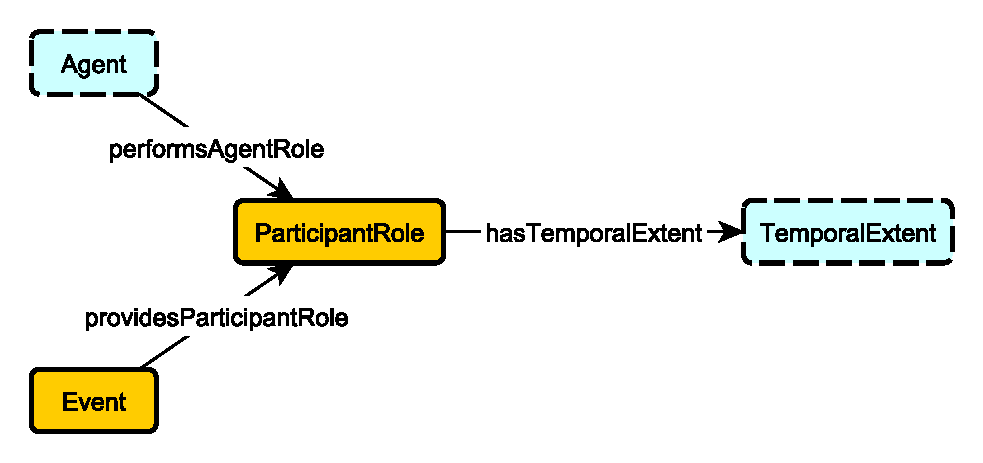
\includegraphics[width=.8\textwidth]{figures/participantrole}
\end{center}
\caption{Schema Diagram for the ParticipantRole Pattern. The visual notation is explained in Chapter \ref{chap:prelims}.}
\label{fig:ParticipantRole}
\end{figure}
\subsection{Summary}
\label{sum:ParticipantRole}
%%%%%%%%%%%%%%%%%%%%%%%%%%%%
The \textsf{ParticipantRole} Pattern is a specialization of the \textsf{AgentRole} Pattern, which can be found in Section \ref{sec:AgentRole}; many axioms are inherited due to this. We include it for convenience as it occurs frequently in our modelling experiences. This pattern has additional synergies with the \textsf{Event} Pattern \cite{event,enslave}.

%%%%%%%%%%%%%%%%%%%%%%%%%%%%%%%%%%%%%%%%%%%%%%%%%%%%%%%%
\subsection{Axiomatization}
\label{axs:ParticipantRole}
%%%%%%%%%%%%%%%%%%%%%%%%%%%%
\begin{align}
\textsf{ParticipantRole} &\sqsubseteq \textsf{AgentRole} \\
\textsf{providesParticipantRole} &\sqsubseteq \textsf{providesAgentRole} \\
\top &\sqsubseteq \forall \textsf{providesParticipantRole.ParticipantRole} 
\end{align}

%%%%%%%%%%%%%%%%%%%%%%%%%%%%%%%%%%%%%%%%%%%%%%%%%%%%%%%%
\subsection{Explanations}
\label{exp:ParticipantRole}
%%%%%%%%%%%%%%%%%%%%%%%%%%%%
\begin{enumerate}
\item Subclass: every \textsf{ParticipantRole} is an \textsf{AgentRole}.
\item Subproperty: \textsf{providesParticipantRole} is a subproperty of \textsf{providesAgentRole}.
\item Range: the range of \textsf{providesParticipantRole} is \textsf{ParticipantRole}.
\end{enumerate}

%%%%%%%%%%%%%%%%%%%%%%%%%%%%%%%%%%%%%%%%%%%%%%%%%%%%%%%%
\subsection{Competency Question}
\label{cqs:ParticipantRole}
%%%%%%%%%%%%%%%%%%%%%%%%%%%%
\begin{enumerate}[CQ1.]
\item Who were the participants in this event?
\item Which students attended the lecture?
\item Who were the passengers on the cruise?
\end{enumerate}

\newpage
%%%%%%%%%%%%%%%%%%%%%%%%%%%%%%%%%%%%%%%%%%%%%%%%%%%%%%%%
% End Section
%%%%%%%%%%%%%%%%%%%%%%%%%%%%%%%%%%%%%%%%%%%%%%%%%%%%%%%%
%%%%%%%%%%%%%%%%%%%%%%%%%%%%%%%%%%%%%%%%%%%%%%%%%%%%%%%%